\subsection{Arduino}
\noindent Initial interfacing to the sensors was performed using the Arduino integrated development environment. Because of its ease of access and abstraction, this has become the preferred programming tool for the FORWARD system. The Arduino IDE provides many useful packaging tools to allow us complete and efficient flashing of the ESP and AMB82-MINI boards. We can simply install the needed libraries, include them in our code, and then click the program button within the IDE. \noindent Initial interfacing to the sensors was performed using the Arduino integrated development environment with an Arduino Uno board. Because of its ease of access and abstraction, this has become the preferred programming tool for the FORWARD system. The Arduino IDE has the built-in serial plotter, which can be integrated with MATLAB for use of a polar plot showing the field-of-vision. The Arduino IDE will continue to be used as a development tool going into Senior Design II, while the Arduino Uno will not, as the FORWARD team fully transitions to the ESP32.\\

\noindent The Arduino IDE is also built upon C/C++ which is a comfortable programming language for our team, with an intuitive approach for programming our system. Not only this, but due to the large amount of support that the IDE receives from Arduino, there are many example codes to assist us in achieving specific functionalities for our purposes. This provided much help for our team in designing the object detection code. \\

\subsection{Detection Subsystem}
\noindent Recall the requirements of the detection subsystem. It should be able to detect objects at least 3 meters away and within a 15 degree aspect angle. It also should detect walker instability up to 10 degrees in pitch angle. It should detect hazards with an accuracy of at least 80\%. Finally, feedback latency should not exceed 100 milliseconds to keep the user safe.\\

\noindent Let us also define the input and output of the obstacle detection subsystem. The input is energy return from the environment, supplied to 5 different points on the walker frame, as well as accelerometer and magnetometer data outputs describing the attitude of the walker itself. The output is somewhat joint with the obstacle identification system, as it helps to generate velocity motor commands for both speed and turn angle. Detection and identification are the FORWARD system inputs, and avoidance is the output.

\subsubsection{Addressing Stretch Goals}
\noindent The range sensors are mounted on the frame perpendicularly to obstacles. In other words, the direction of the energy transmitted is parallel to the ground. However, the question of maximizing capability of detecting obstacles at the wheel level, and to prevent ignorance of more dangerous and deceptive hazards such as ledges or step-downs is raised. The monostatic ones will be mounted on the legs near the wheels, front-facing, while the multistatic are used for lateral detections.\\

\noindent To achieve \textit{curb lifting}, we rely on successful classification of an approaching ledge scenario by the recognition image processing, which we foresee could be challenging due to the non-distinctness of curbs, and the difficulty the sensors will have detecting them. When the front wheels are about to make contact, we can use the audio feedback to prompt the user to push down on the handlebars to raise the front wheels, then also give haptic feedback once they have placed them onto the new ground. The user is then prompted to move forward, raising the rear wheels and placing them atop the curb in the same manner as before, confirmed by haptic vibrations.\\

\noindent To achieve \textit{tipover stabilization}, we can monitor for a sudden positive delta in the pitch angle reading of the IMU. It's rate of change would need to be fast enough to distinguish from merely a change of terrain, when in fact, the user is still stable. The rapid change of pace means the user has fallen forwards while still holding the handlebars. By applying the emergency brake, friction between the rear wheels (the front wheels have reared up) can help convert the rollator into a crutch. Potentially, commanding the motors to spin backward to prop the user up to brace their fall could work too, but intense testing is required.\\

\subsubsection{Incline and Decline Stability}
\noindent The simple function fulfilled by the inclusion and integration of the IMU is stability. By monitoring the pitch angle of the walker, we know whether the user is at risk of falling over.\\

\begin{figure}[H]
	\centering
	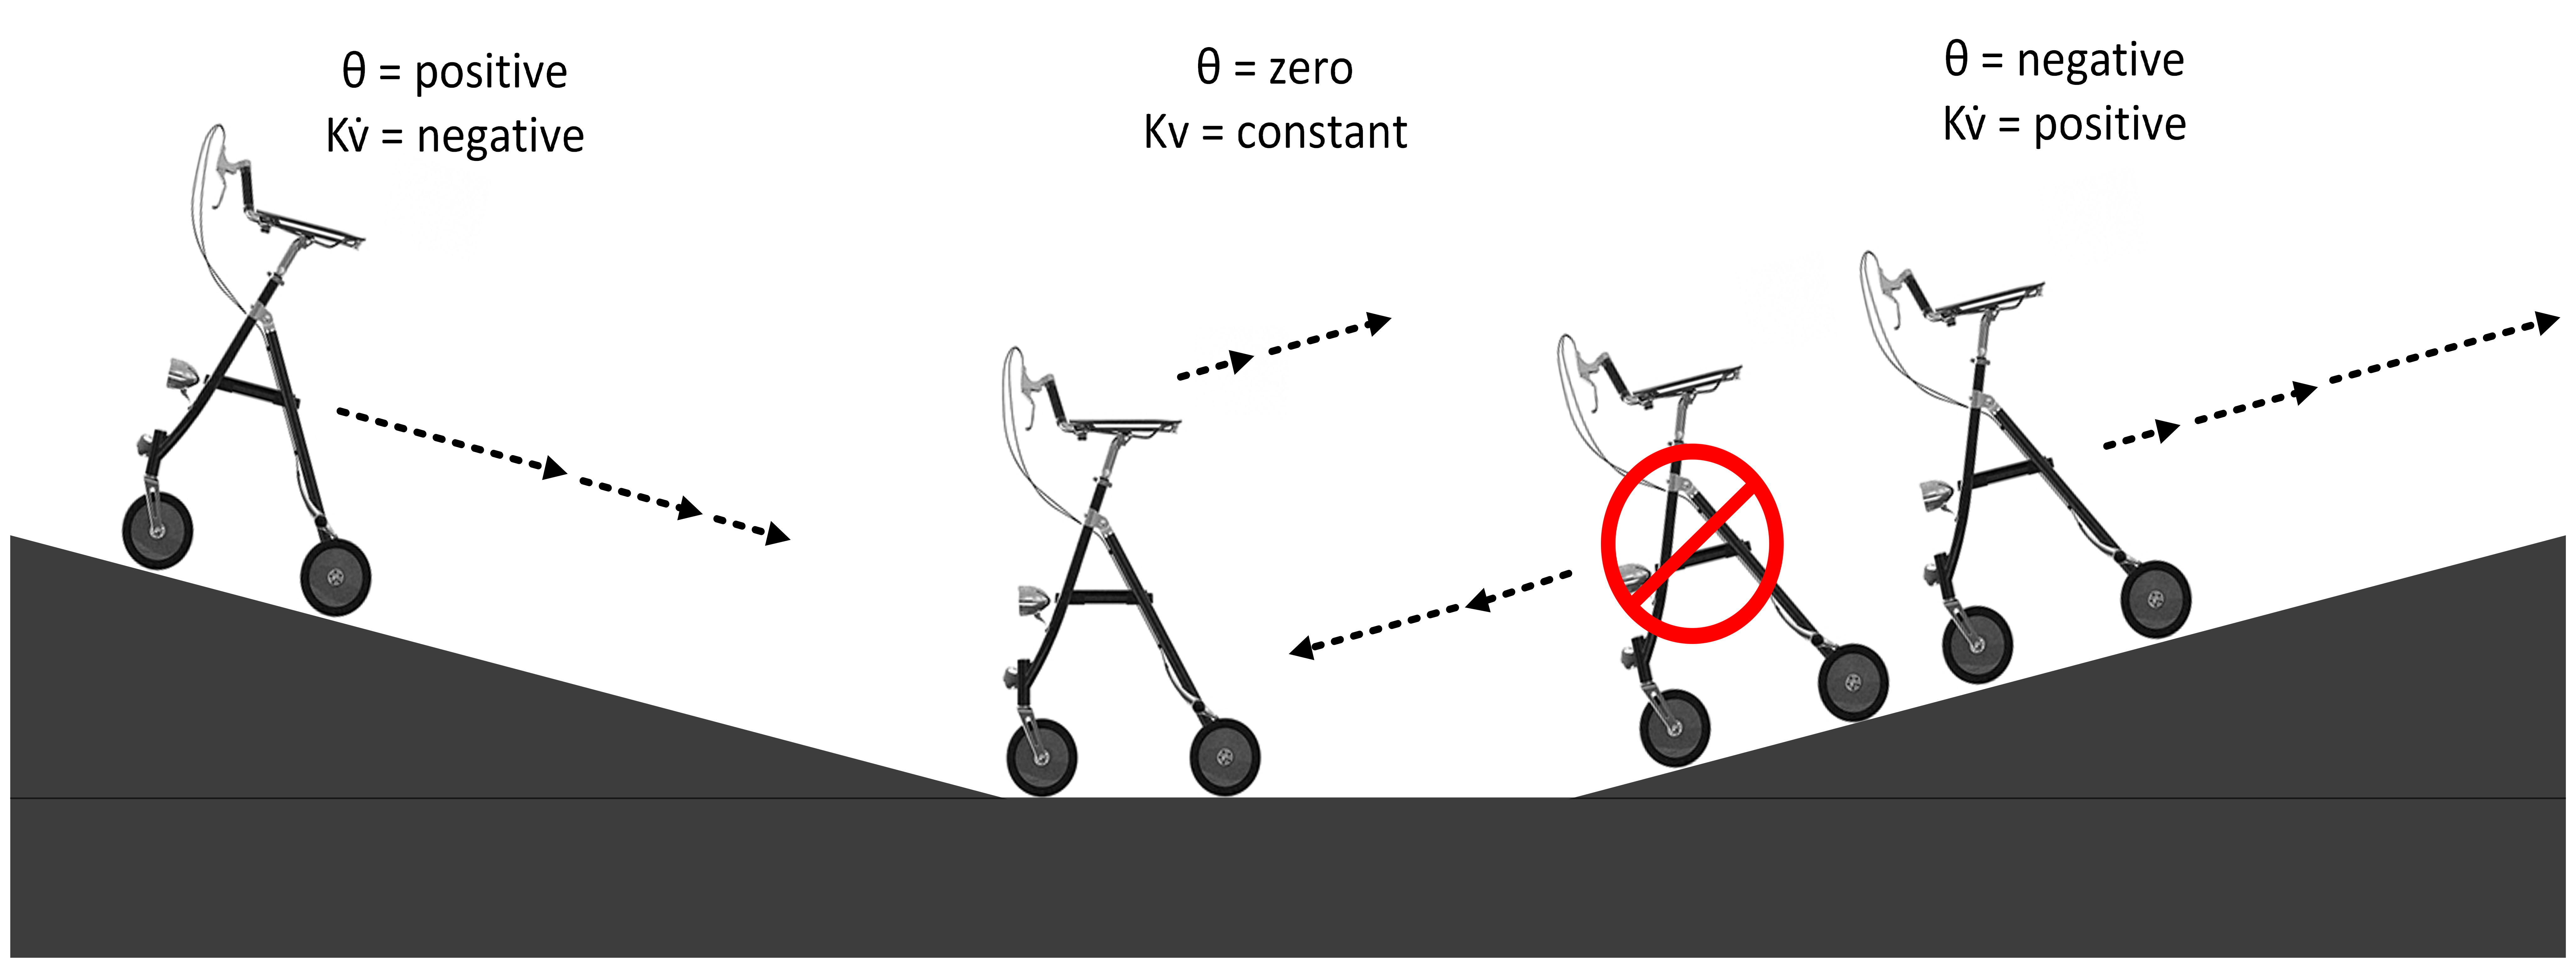
\includegraphics[width=\textwidth]{./Images/Incline-Decline-Stability.png}
	\caption{\label{fig:slope-stability}Stability on Slopes}
\end{figure}

\subsubsection{Tilting Stability}
\noindent The IMU reads data from three different angles: pitch, yaw, and roll. We discussed previously under Incline and Decline Stability how we will use the pitch angle to prevent the rollator from rolling back on the user. We will also apply the roll angle to determine if the user is leaning too heavily on one side of the walker. If, for example, the user transfers the majority of their body weight to the right handlebar, the left side of the walker will tilt upward. This will increase the roll angle on the IMU (which should be zero for a stable system). The user will then be alerted through audio feedback that the walker is tipping. This feedback will be necessary to prevent the user from entirely capsizing the walker.\\

\begin{figure}[H]
	\centering
	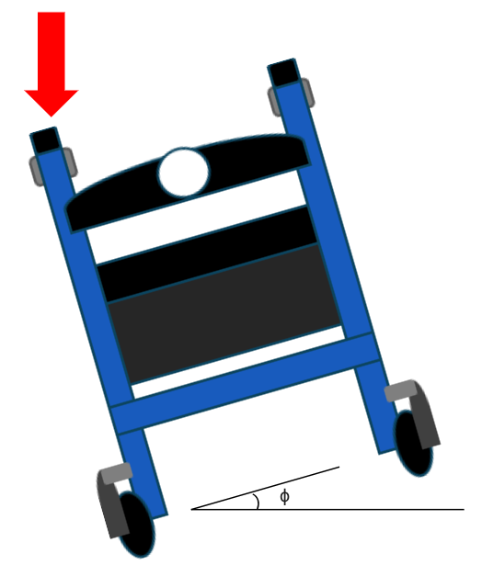
\includegraphics[width=.3\textwidth]{./Images/roll.png}
	\caption{\label{fig:roll}Stability in Tilting}
\end{figure}

\subsubsection{Sonar Pulse Interference}
\noindent One important note to consider is interference of the ultrasonic pulses. Being that FORWARD uses four of them, it is important to make sure the receivers do not receive each others emitted energy reflections. Ultrasonics are directional, so by pointing the multistatic sensors to the left and right sides of the rollator to monitor passing or approaching obstacles, we decouple them from the monostatic. However, the front-facing sensors are only separated by the length of the axle, meaning these will need to be triggered sequentially to avoid interference. This can be implemented simply in Arduino by separate digital write statements with a delay proportional to the one way pulse return duration. Actually, we observed this occurring during the first testing for the demo video, and troubleshooting is currently under way.\\

\subsubsection{Sensor Fusion}
\noindent How do we make sense of the range detection made at all five points of the front-face of the walker? How do we combine that with pixel data of the corners of an object detection made by the camera? We can generally perceive depth by averaging the 4 coordinates, where closer is a higher average. We also know whether an obstacle is on the left or right side ahead based on which ranges are lower the maximum. We have to take into account the dead zones. The IMU will also provide us with key information about the walker body itself, allowing for certain counter measures to be made to increase stability. With all of this information available on the network, we can build algorithms to guide the way forward, as discussed in the following chapter.\\

\noindent As noted, the ESP32 development board supports all the sensors and the camera simultaneously without the need of multiplexing. The setup pictured below in figure \ref{fig:bb-test} has the IMU and LiDAR on an I2C bus, and the ultrasonic sensors routed to GPIO pins. A table of the varying assignments, labels, and voltage requirements would be provided for the topology in figure \ref{fig:bb-test}, but it is forbidden by the UCF ECE guidelines. Suffice it to say, the IMU requires 3.3V, the TFLuna LiDAR requires 5V, and both variants of the ultrasonic can support either voltage.\\
\begin{figure}[H]
	\centering
	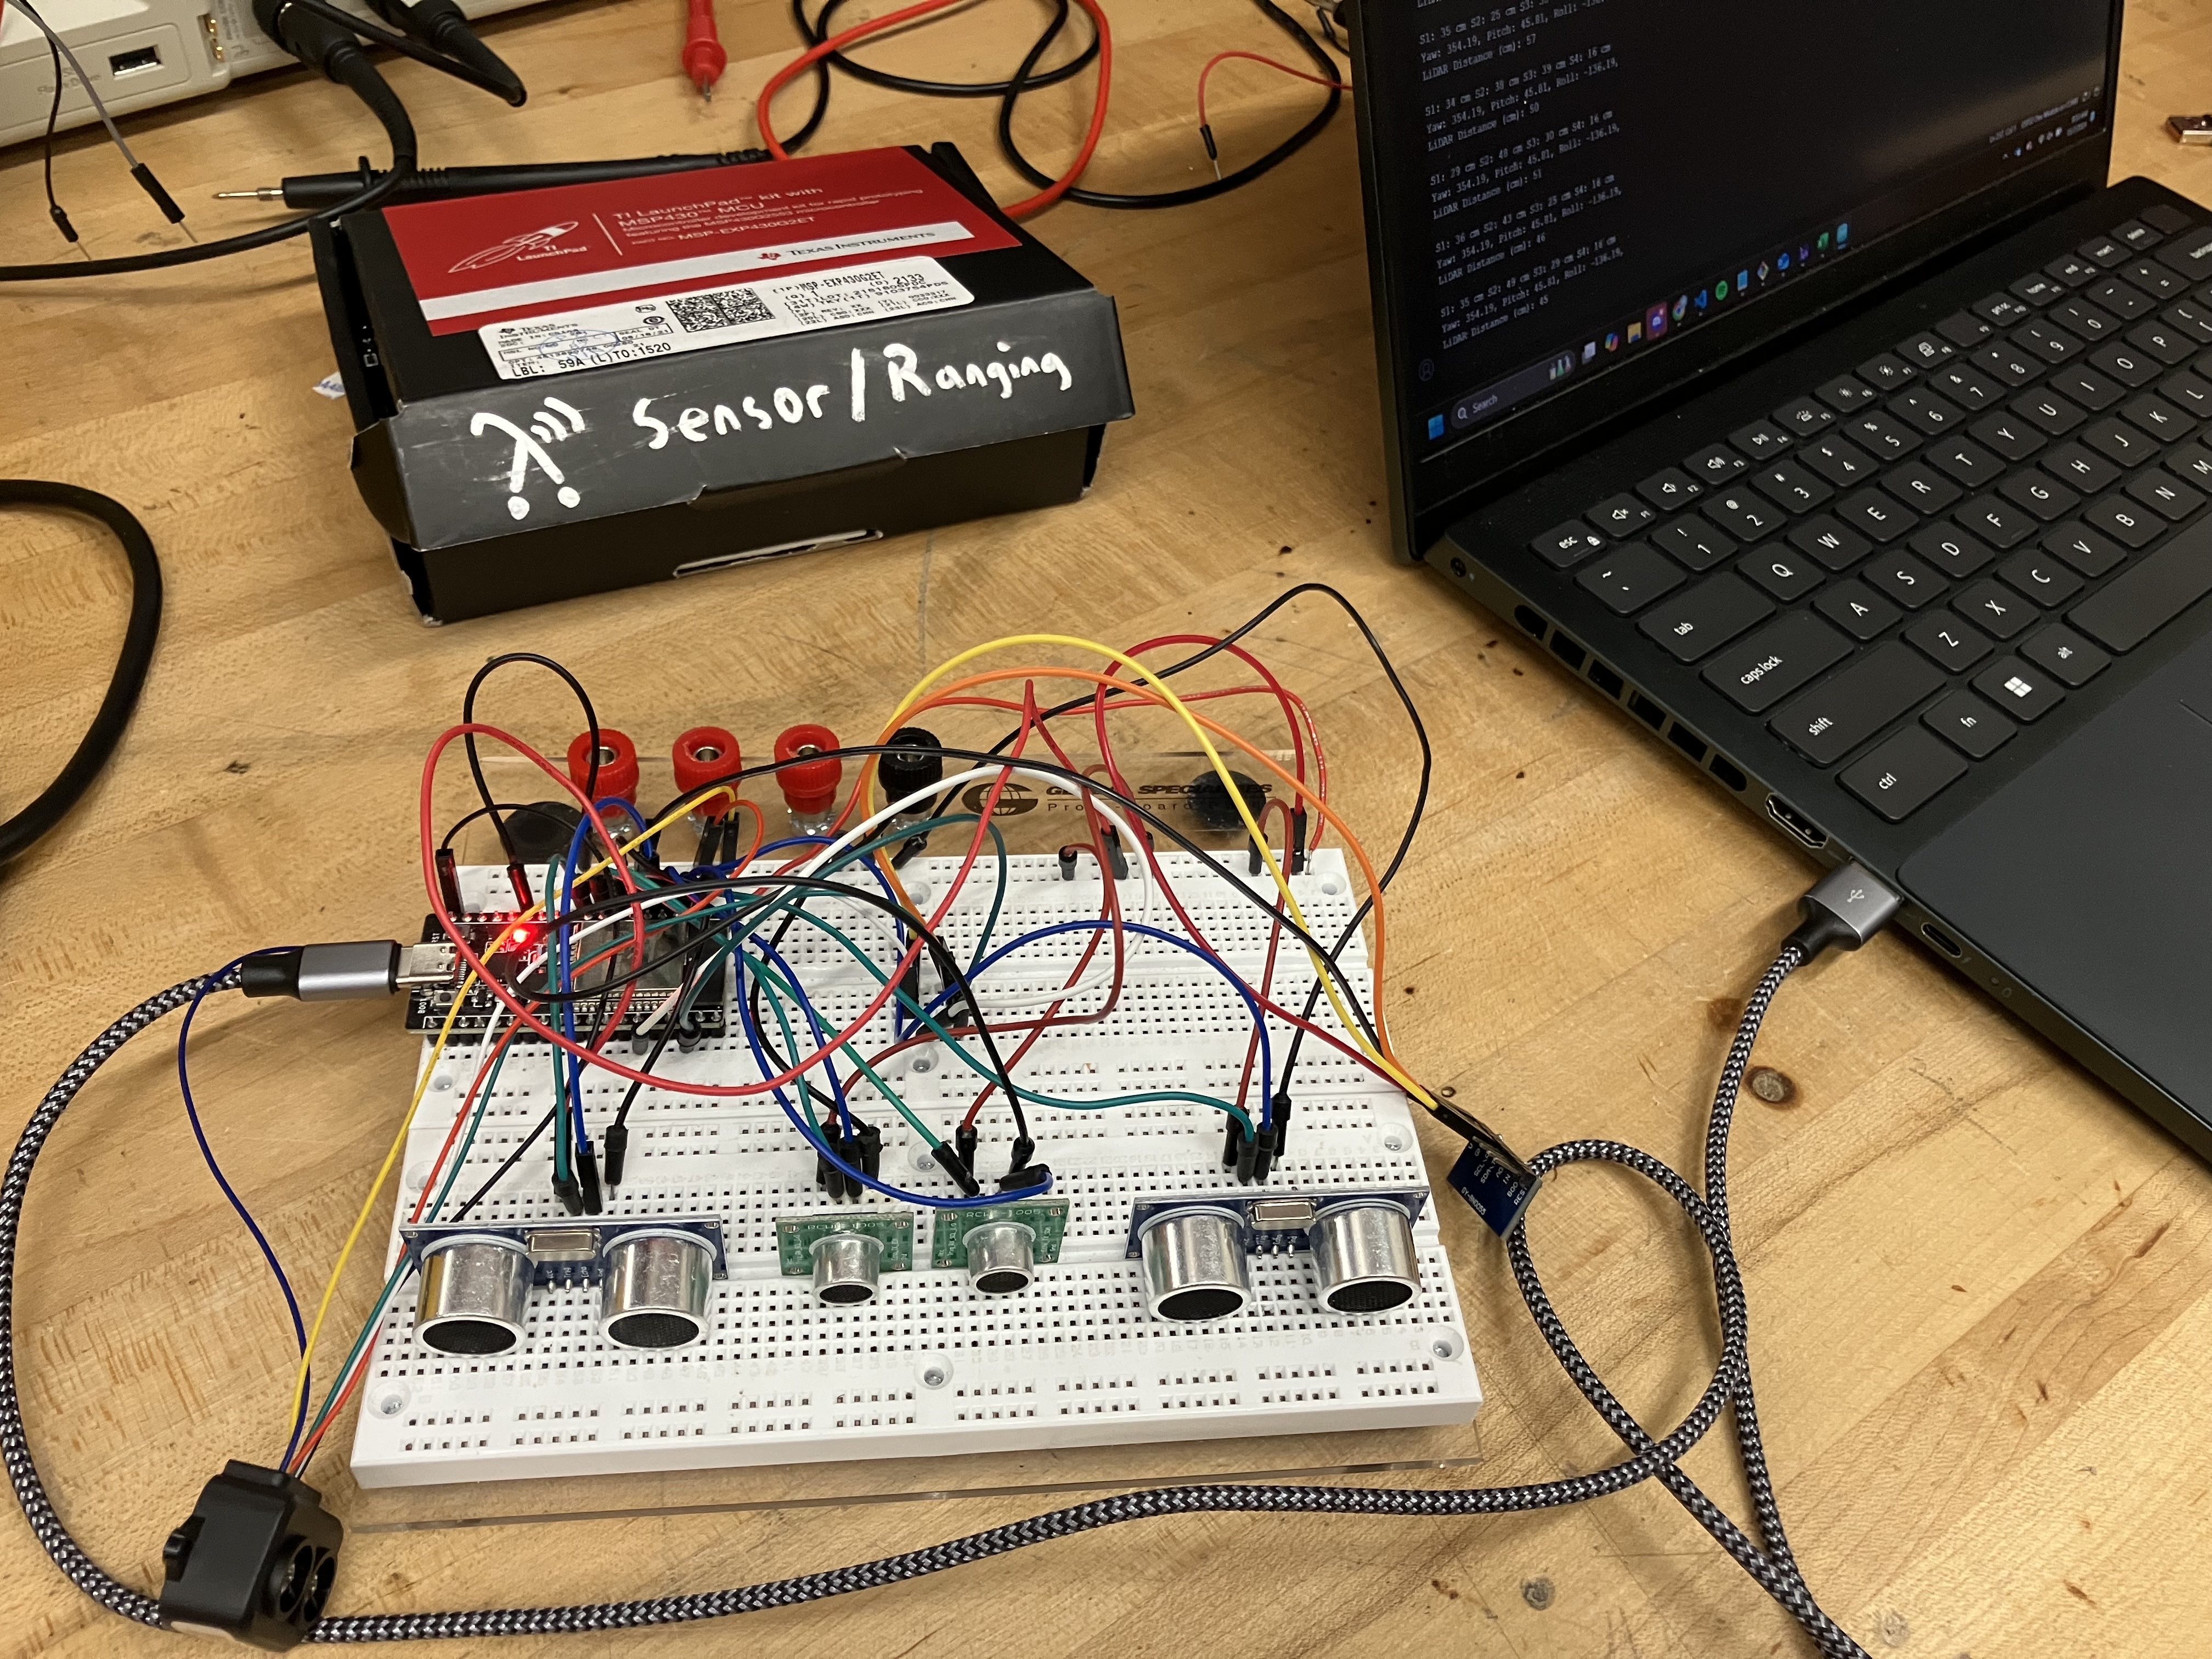
\includegraphics[width=0.5\textwidth]{./Images/breadboard-test.jpg}
	\caption{\label{fig:bb-test}Breadboard w/ Ultrasonics, and IMU \& LiDAR I2C Bus}
\end{figure}

